\documentclass[a4paper,10pt]{article}
\usepackage[utf8]{inputenc}
\usepackage[T1]{fontenc}
\usepackage[margin=1in]{geometry}
\usepackage{enumitem}
\usepackage{hyperref}
\usepackage{graphicx}
\usepackage{xcolor}
\usepackage{titlesec}
\usepackage[english]{babel}
\usepackage{helvet}
\renewcommand{\familydefault}{\sfdefault}

\definecolor{sectioncolor}{RGB}{44,62,80}
\definecolor{bubblebg}{RGB}{239,239,239}
\definecolor{bubbletext}{RGB}{51,51,51}

\titleformat{\section}[block]
    {\color{sectioncolor}\normalfont\LARGE\bfseries}
    {}{0ptx}{}

\setlist[itemize,1]{leftmargin=\dimexpr 26pt-.10in, label=\textbullet, noitemsep}

\usepackage{tikz}
\newcommand{\bubble}[1]{%
    \tikz[baseline=(text.base)]{
        \node[draw=none, fill=bubblebg, rounded corners=8pt, inner xsep=6pt, inner ysep=2pt] (text) {\textcolor{bubbletext}{\strut#1}};
    }%
}

\begin{document}

% Header
\begin{center}
    {\LARGE \textbf{Nathan Fitger}}\\[0.5em]
    \textit{MSc Student in Artificial Intelligence at the University of Bordeaux}\\[1em]
    \hspace{1.5em}\href{mailto:nath.fitger@gmail.com}{nath.fitger@gmail.com} \textbar\ 
    \href{https://www.linkedin.com/in/nfitger/}{
\includegraphics[height=1em]{ressources/logo-linkedin.png} Nathan Fitger} \textbar\ 
    \href{https://github.com/0xNatgan}{
\includegraphics[height=1em]{ressources/github.png} 0xNatgan} \textbar\ 
    {
\includegraphics[height=1em]{ressources/appel.png} +33 7 81 61 31 02}\\
    \href{https://0xNatgan.github.io}{Link to my online resume: 0xNatgan.github.io}
\end{center}

\vspace{1em}

% Photo (top left corner)
\begin{picture}(0,0)
    \put(-20,0){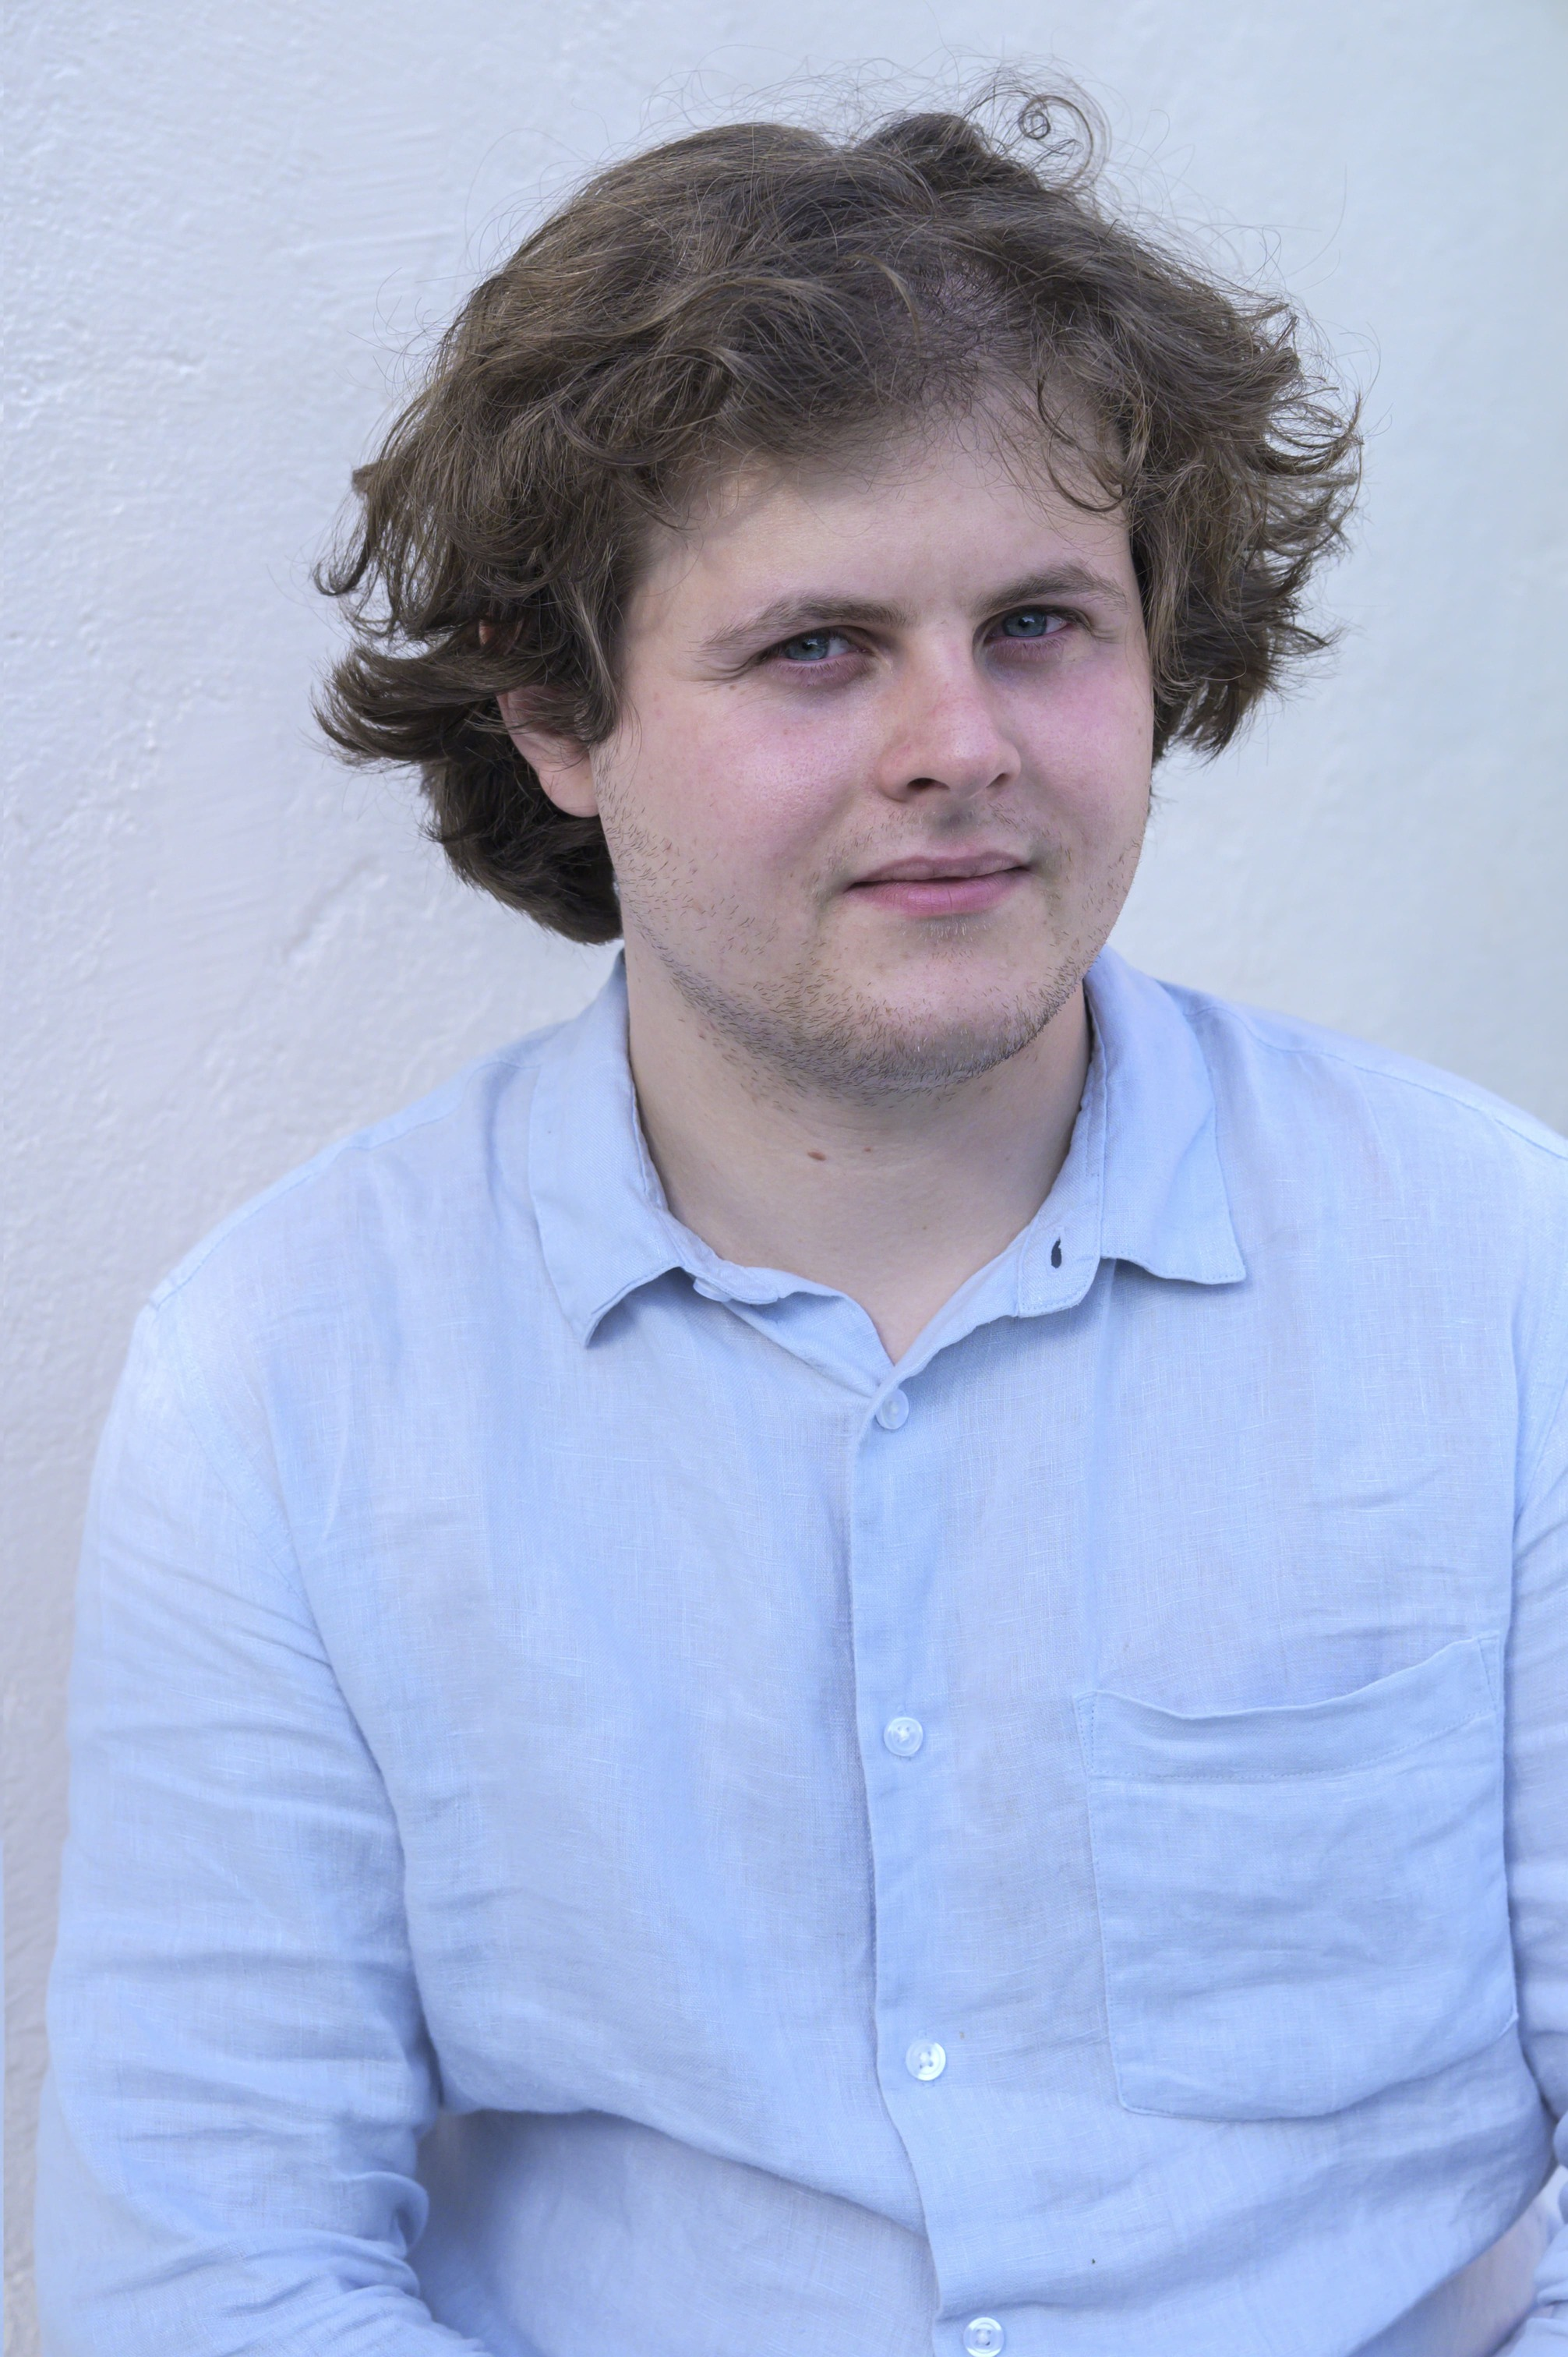
\includegraphics[width=2.2cm]{ressources/photo_cv.jpg}}
\end{picture}

% Profile
\section*{Profile}
Artificial intelligence student passionate about computer science and new technologies. I am looking for a six-month internship in the field of AI starting from March 2026.

Having explored various fields such as robotics, web development, and cybersecurity before specializing in AI, I have acquired solid skills in programming and data analysis. I am always looking for new challenges to expand my knowledge.

Through my experiences as an IT fleet manager, instructor and designer of IT and robotics training courses, CTF participant, and AI intern, I have learned to work in teams and to master new tools and programming languages to adapt to required tasks.

% Skills
\section*{Skills}

\noindent \bubble{Python}  \bubble{Scikit-learn} \bubble{Pytorch} \bubble{LSP-servers} \bubble{C} \bubble{C++} \bubble{Java} \bubble{API} \bubble{Machine Learning} \bubble{Deep Learning}  \bubble{Docker} \bubble{Git} \bubble{CTF} \bubble{AI} \bubble{Open source} \bubble{RAG} \bubble{Neural Networks} \bubble{Language Models} \bubble{SQL} \bubble{HTML} \bubble{CSS} \bubble{GLPI} \bubble{Cybersecurity} \bubble{Robotics} \bubble{Linux} \bubble{Mkdocs} \bubble{Web}  \\
\newline
\noindent\textbf{Languages:} English C1+ (Linguaskill) \textbar\ German B2\\
\noindent\textbf{Driving licence (Permis B)}\\
\noindent\textbf{Geographic mobility:} Available to opportunity in France and abroad

% Experience
\section*{Experience}
\noindent\textbf{AI Internship -- Gertrude.fr -- Intelligent Transportation System}\\ \hfill \textit{May 2025 -- July 2025, Bordeaux}
\begin{itemize}
    \item Developed a code documentation tool using language models and RAG.
    \item Advised on the integration of artificial intelligence tools for the company.
    \item Participated in AI research projects related to urban traffic.
\end{itemize}

\noindent\textbf{Volunteer IT fleet management and Treasurer -- Jeunes sciences Bordeaux}\\ \hfill \textit{2019 -- 2025, Bordeaux}
\begin{itemize}
    \item Management and maintenance of the IT fleet using GLPI
    \item Technical support for users
    \item Maintenance of computer equipment
\end{itemize}

\noindent\textbf{CS and Robotics course designer and instructor -- Jeunes sciences Bordeaux}\\ \hfill \textit{2019 -- 2025, Bordeaux}
\begin{itemize}
    \item Designed and led robotics and computer science courses for young people aged 8 to 17
\end{itemize}

\noindent\textbf{Summer jobs in catering}\\ \hfill \textit{Summer 2021 to 2024, Bordeaux}
\begin{itemize}
    \item 2021: Eklo Bordeaux -- Runner, floor service, order taking and bartender
    \item 2023: Heiko Poké Bègles -- All-purpose restaurant employee
    \item 2024: Island Poké -- All-purpose restaurant employee
\end{itemize}

% Education
\section*{Education}
\noindent\textbf{Master's in Artificial Intelligence -- University of Bordeaux} \hfill \textit{2024 -- 2026}\\
\indent Master's in Artificial Intelligence. Specialization: Advanced Databases\\

\noindent\textbf{Bachelor's in Computer Science -- University of Bordeaux} \hfill \textit{2020 -- 2024}\\

\noindent\textbf{Web Developer Training -- Le Wagon} \hfill \textit{Sept. -- Nov. 2021}\\
\indent Intensive web development bootcamp.\\

\noindent\textbf{Scientific Baccalaureate -- Lycée Vaclav Havel} \hfill \textit{2019--2020}\\


% Projects
\section*{Projects}
\noindent\textbf{DocGen\_LLM} (\href{https://github.com/0xNatgan/DocGen_LLM}{github.com/0xNatgan/DocGen\_LLM})

\indent Code documentation generation tool using language models and RAG.\\

\noindent
\bubble{Python} \bubble{Docker} \bubble{Language Servers} \bubble{LLM} \bubble{RAG} \bubble{documentation} \bubble{mkdocs} \bubble{Markdown} \bubble{HTML} \bubble{open source} \bubble{AI}\\

\begin{itemize}
    \item Main goal: To generate code documentation in an automated and language-agnostic way for projects lacking clear or existing documentation.
    \item DocGen\_LLM is a code documentation generation tool that uses language models in combination with language servers to generate clear and concise documentation for an entire codebase. It is designed to be programming-language agnostic. The tool easily integrates with documentation tools like mkdocs and allows generating documentation to be added to the code or used in external documentation in Markdown or HTML format.
\end{itemize}
\noindent\textbf{TCL Language Server} (\href{https://github.com/0xNatgan/tcl-lsp}{github.com/0xNatgan/tcl-lsp})

Simple TCL language server for code analysis.\\

\noindent
\bubble{TCL} \bubble{Language Server} \bubble{TCP} \bubble{stdin/out}\\

\begin{itemize}
    \item Main goal: To analyze a TCL project, I developed a language server to facilitate this task and make it compatible with my DocGen\_LLM project.
    \item This language server allows the analysis of TCL code and the extraction of information according to the LSP standard. This project is a simple implementation of a TCL language server with the following capabilities: symbol extraction, definition lookup, and reference search. The project includes both stdin/out and TCP interfaces.\\
\end{itemize}

\noindent\textbf{Quoridor}

Quoridor board game developed in Java with a graphical interface and AIs. Project made during my studies at the University of Bordeaux.\\

\noindent
\bubble{Java} \bubble{AI} \bubble{GUI} \bubble{JavaFx} \bubble{Junit} \bubble{JavaDoc} \bubble{Maven} \bubble{CLI} \\

\begin{itemize}
    \item Main goal: To develop a Quoridor board game in Java with a graphical interface and AIs for the user to play against. The implementation should include a user-friendly GUI, AI opponents with varying difficulty levels, a robust game engine and should respect industry standards such as clean tests and complete documentations.
    \item This project includes an implementation of the Quoridor game with a graphical interface in Java and AIs for the user to play against, as well as advanced statistics on the AI algorithms used.
\end{itemize}

\end{document}